\documentclass[11pt]{article}
\usepackage[margin=1cm]{geometry}
\usepackage[portuguese]{babel}
\usepackage[utf8]{inputenc}
\usepackage{hyperref}
\usepackage{indentfirst}
\usepackage{subfig}
\usepackage{listings}
\usepackage{color}

\definecolor{dkgreen}{rgb}{0,0.6,0}
\definecolor{gray}{rgb}{0.5,0.5,0.5}
\definecolor{mauve}{rgb}{0.58,0,0.82}

\lstdefinestyle{mystyle}{
  commentstyle=\color{codegreen},
  % keywordstyle=\color{magenta},
  % stringstyle=\color{codepurple},
  basicstyle=\ttfamily\footnotesize,
  breakatwhitespace=false,
  breaklines=true,
  captionpos=b,
  keepspaces=true,
  numbers=left,
  numbersep=5pt,
  showspaces=false,
  showstringspaces=false,
  showtabs=false,
  tabsize=2
}
\lstset{style=mystyle}

\urlstyle{same}
\pagenumbering{gobble}
%\usepackage{multicol}
\hypersetup{
  colorlinks=true,
  linkcolor=black,
  filecolor=magenta,      
  urlcolor=blue,
  citecolor=black,
}
\usepackage[backend=bibtex]{biblatex}
\usepackage{graphicx}
\usepackage{tikz}
\pagestyle{plain}

\newcommand{\gaspar}{Diogo Gaspar, 99207}

\begin{document}
\begin{center}
{\huge{Exercício 6 - Projeto Computacional PE 2022}} \\
\vspace{1.5mm}
{\large{\gaspar}} \\
\end{center}

Consideremos como premissas que foram fixadas uma semente em 1896, três
tamanhos de amostras (respetivamente 4, 27, e 70) e um intervalo contínuo [4,8].
O objetivo deste exercício passa por gerar 500 amostras com distribuição uniforme
contínua para cada tamanho supra-mencionado. De seguida, calcular a média de cada uma
das amostras (obtendo, assim, os valores da distribuição da média associada às amostras
de cada tamanho), e ilustrar, através de um histograma de densidade, a
relação entre os valores obtidos para a distribuição das médias e a distribuição normal
das mesmas, considerando valor esperado E(X) e a variância Var(X)/n.

$$
E(X) = \frac{(4 + 8)}{2}
$$
$$
\forall_{n \in \{4, 27, 70\}}, \quad \sigma^2 = \frac{Var(X)}{n} \leftrightarrow \sigma = \sqrt{Var(X) / n} = \sqrt{\frac{(8 - 4)^2}{12n}}
$$

\vspace{0.5mm}
Para tal, recorreu-se ao seguinte trecho de código \texttt{R} (utilizando as bibliotecas \texttt{ggplot2, gridExtra} e \texttt{purrr}):

\begin{lstlisting}[language=R]
  set.seed(1896)
  n_values <- c(4, 27, 70)
  sample_amount <- 500
  a <- 4
  b <- 8
  expected_value <- (b + a) / 2

  calc_sd <- function(n) {
    return (sqrt(((b - a)**2) / (n * 12)))
  }
  calc_means <- function(n) {
    means <- c()
    for (i in 1:sample_amount) {
      means <- c(means, mean(runif(n, 4, 8)))
    }
    return (means)
  }

  calc_plot <- function(n) {
    means <- calc_means(n)
    df <- data.frame(means)
    ggplot(df, aes(x = means)) +
      geom_histogram(aes(y=..density..), color="white", fill="orange", bins=40) +
      stat_function(fun=dnorm, args=list(mean=expected_value, sd=calc_sd(n))) +
      theme_bw() +
      labs(x = paste("Distribuição da média, n =", n), y = "Densidade") +
      scale_y_continuous(breaks = seq(0, 5, .2))
  }

  plots <- map(n_values, calc_plot)
  grid.arrange(grobs = plots, layout_matrix = matrix(c(3,1,3,2), nrow = 2))
\end{lstlisting}

\begin{tikzpicture}[remember picture, overlay]
  \node [shift={(-6cm, -13.25cm)}] at (current page.north east)
    { 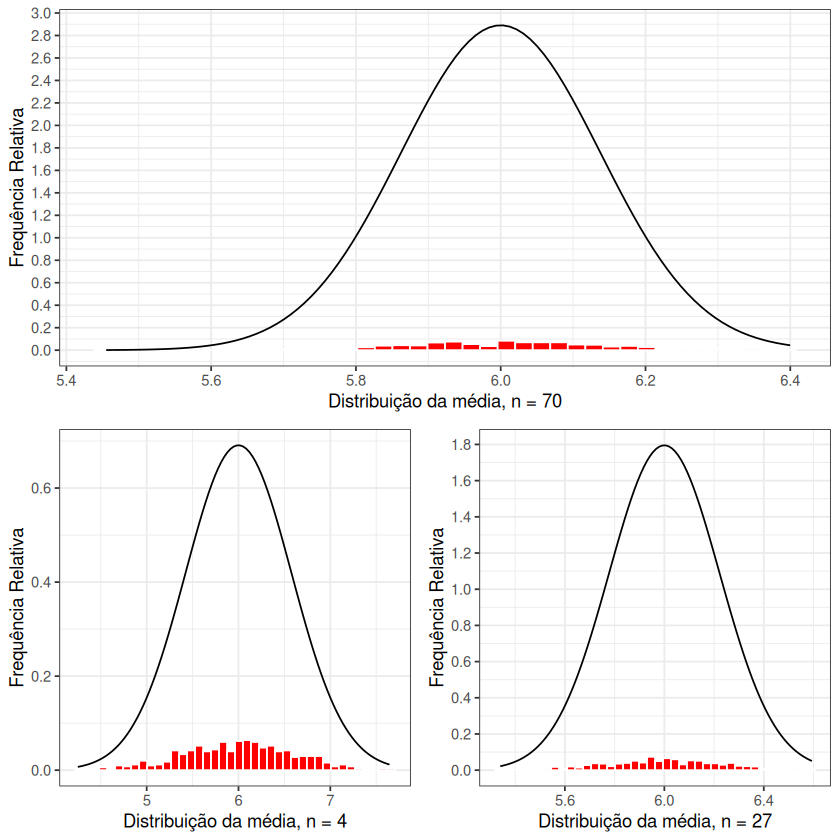
\includegraphics[scale = 0.45]{../imgs/exercise-6.png} };
\end{tikzpicture}

Note-se, tal como esperado, que o pico da distribuição normal encontra-se, em todos
os histogramas, no valor 6, decaindo suavemente para os lados. Mais, o tamanho da amostra aparenta ser
inversamente proporcional ao desvio padrão.

\end{document}